\section{Appendix B: Overcoming Background Galaxy Contamination}\label{sec:appB}

In this appendix, the probability of failed host galaxy associations for nearby transients with large host offsets due to interloping background galaxies is quantified, and used to evaluate the minimum number of potential hosts that should be stored in a {\tt DIAObect} record. 
For simplicity, this appendix uses the effective radius as the separation distance (Section \ref{ssec:options_Re}).

The 10-year {\tt Object} catalogs will include $\sim$4 billion galaxies with $i<25$ mag across the $\sim$20000 $\rm deg^2$ main survey area, known as the ``gold" sample, especially in the context of weak lensing studies \citedsp{LPM-17}.
However, the 10-year coadded depths will detect galaxies down to 5$\sigma$ limiting magnitudes of 26.1, 27.4, 27.5, 26.8, 26.1, and 24.9 mag in filters {\it ugrizy}; this is $\sim$3 times as many as in the ``gold" sample, or $\sim$10 billion galaxies.
This high density of background galaxies complicates the process for associating large nearby host galaxies with their transients, especially the rare transients in their outskirts.

Consider a transient at $3R_e$ from the center of a nearby galaxy with $z=0.01$ and an effective radius of $R_e = 10$ kpc ($\sim$50 arcsec).
In order for this transient to be associated with it's true host, the separation distance for all {\tt Objects} within a radius of at least $3R_e$, and thus an area of at least $A_{3R_e} = \pi (3R_e)^2 = 0.0052$ $\rm deg^2$, would need to be considered.
Based on the final 10-year number of detected galaxies (10 billion) and the total survey area (20000 deg$^2$), that is $\sim (10^10 / 20000) \times 0.0052 \approx 2600$ galaxies.
Furthermore, the true host galaxy must have a lower separation distance than the $N$ nearest background galaxies, where $N$ is the number of potential hosts that will be listed in the {\tt DIAObject} parameters {\tt potentialHost} and {\tt potentialHostSeparation}.

\begin{figure}[h]
\begin{center}
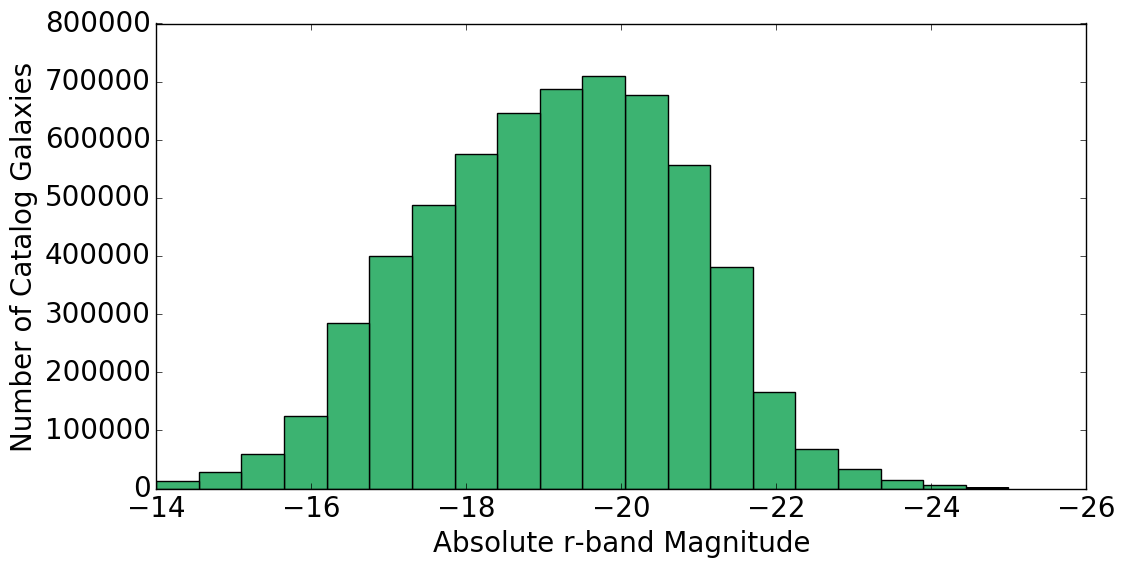
\includegraphics[width=8cm]{hg_Mr_dist.png}
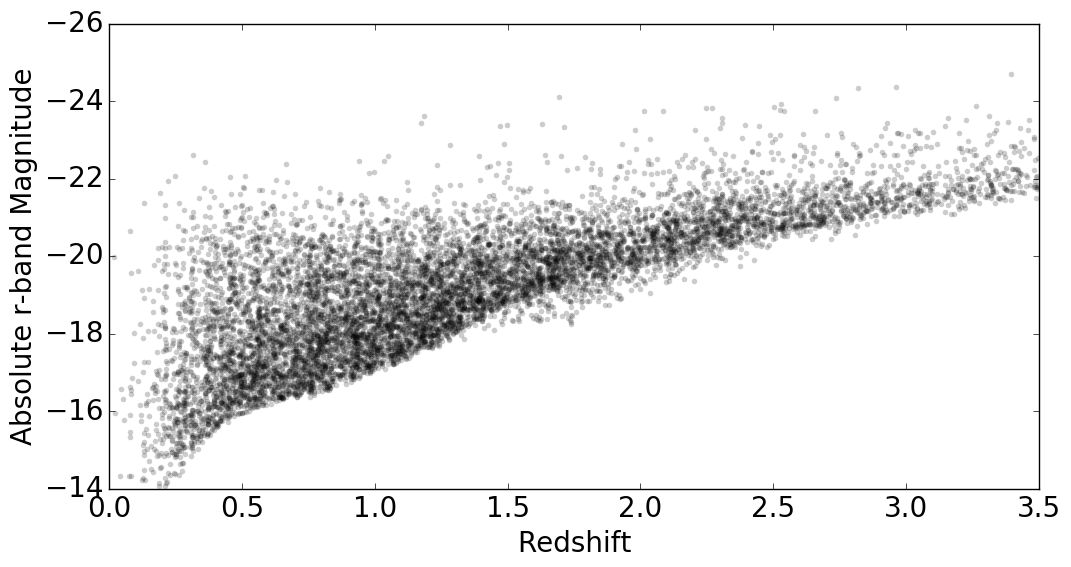
\includegraphics[width=8cm]{hg_Mr_vs_z.png}
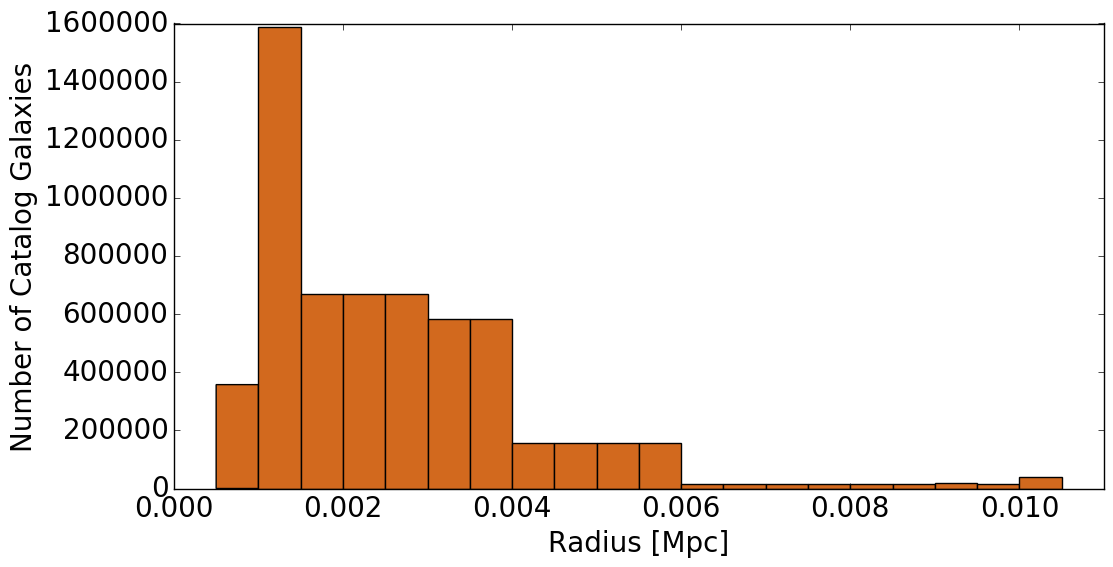
\includegraphics[width=8cm]{hg_rad_dist.png}
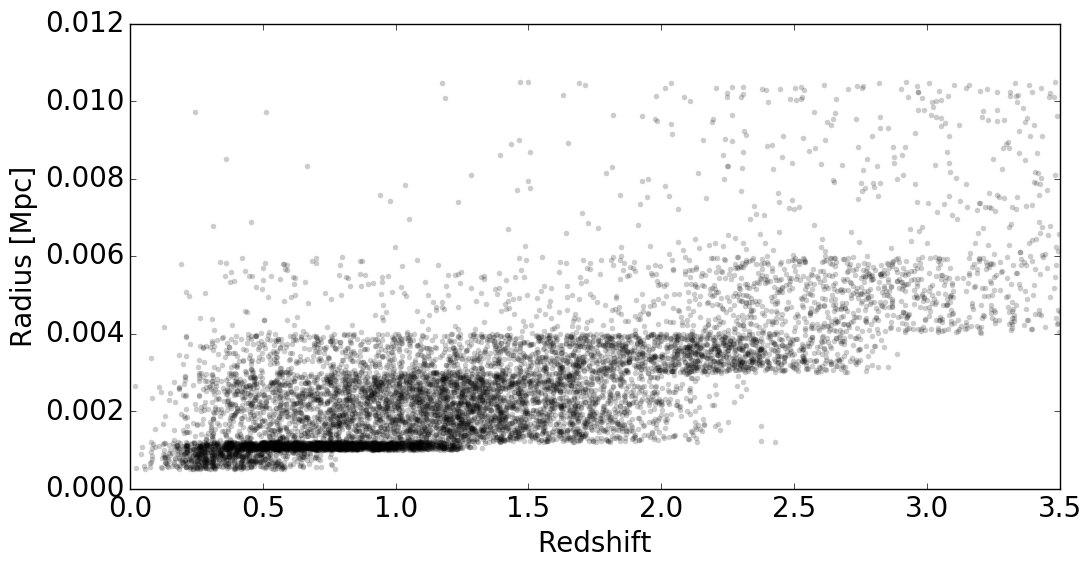
\includegraphics[width=8cm]{hg_rad_vs_z.png}
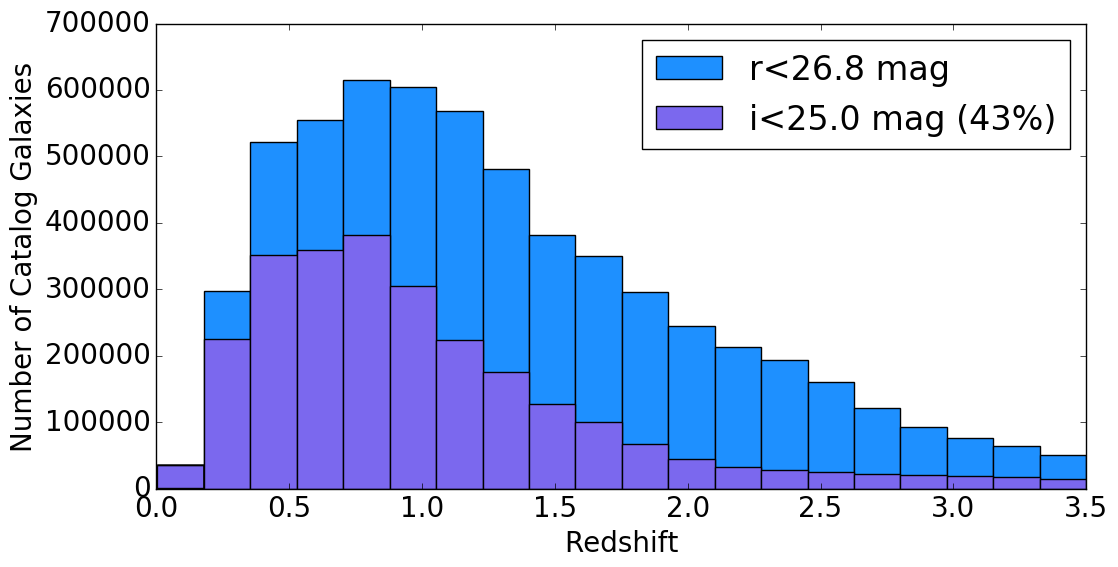
\includegraphics[width=8cm]{hg_z_dist.png}
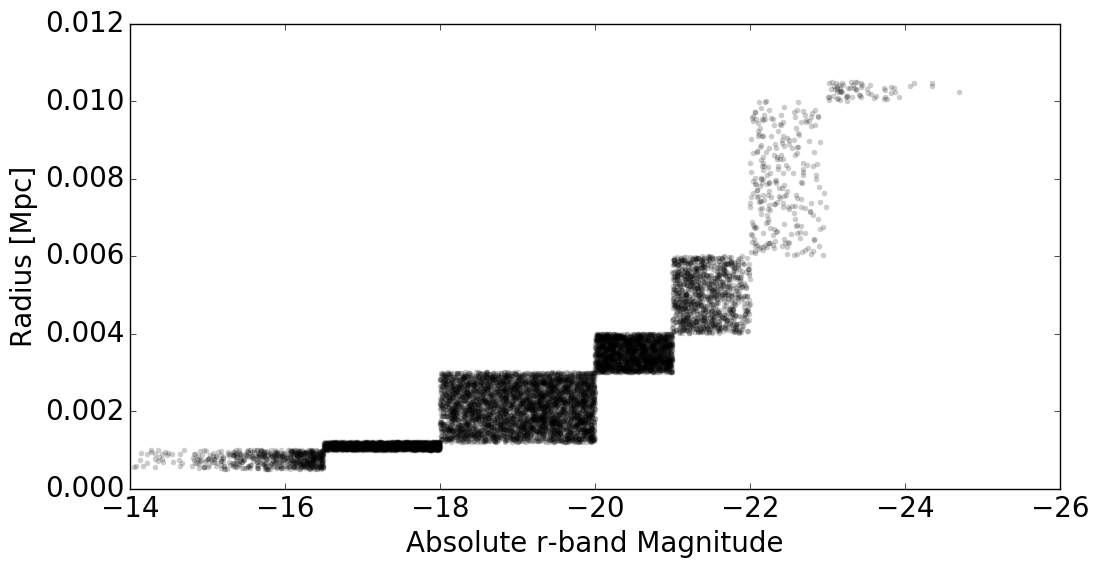
\includegraphics[width=8cm]{hg_rad_vs_Mr.png}
\caption{{\it Left:} Histograms of the synthesized absolute $r$-band intrinsic magnitude (top) and radius (middle) for catalog galaxies, and the simulated galaxy redshifts (bottom). {\it Right:} Correlation with redshift of the synthesized intrinsic magnitude (top) and radius (middle), and the approximate relation between radius and intrinsic magnitude (bottom).  \label{fig:simcat}}
\end{center}
\end{figure}

To investigate the probability of host-association failure for nearby transients, we simulate a mock catalog of randomly distributed random background interloper galaxies.
It is based on the same LSST-like mock galaxy catalog used by \citet{2018AJ....155....1G} for studies of photometric redshifts.
For this experiment the catalog is limited to galaxies with at least a 5$\sigma$ detection in the {\it griz} bands at the projected 10-year depths listed above.
The catalog contains redshifts and apparent {\it ugrizy} magnitudes, which are used to approximate intrinsic absolute $r$-band magnitudes (without $K$-correction, simply using a distance modulus based on redshift and $M_r=m_r-\mu$).
The absolute magnitudes are used to synthesize approximate galaxy radii based on the relationship between absolute magnitude and radius for late-type galaxies defined in Figure 3 of \citet{2003MNRAS.343..978S}.
These synthesized radii are over-estimates because late-types are generally larger than early-types, and because this magnitude-radius relation was defined for SDSS galaxies at lower redshifts than the LSST high-$z$ galaxies it is being applied to.
This is a deliberate choice to overestimate, because it will result in upper limits on the rate of interlopers, which will allow for conservative estimates about the effect of background interlopers.
The characteristics of this crude galaxy catalog are illustrated in Figure \ref{fig:simcat}.

Consider again the large nearby galaxy with $R_e=10$ kpc at a redshift of $z=0.01$, for which the sky area within $3R_e$ is $A(3R_e)=0.0052$ $\rm deg^2$ and contains $\sim$2600 background galaxies.
From the simulated catalog described above, 100 sets of background galaxies are randomly selected.
For each set, the fraction of the nearby galaxy's area which is covered by the area of interloping background galaxies is calculated: $f_A = \sum{A(3R_{e,{\rm bkg}})} / 0.0052$.
This fraction is equivalent to the probability that a transient at $3R_e$ from this large nearby host will be within $3R_{e,{\rm bkg}}$ (i.e., will be closer to) a background interloper.
The probability that this transient is closer to $N$ interlopers than to its true host is $P_{\rm fail} = (f_A)^N$.
This is the probability of a failed host association, where ``failed" means that the {\tt DIAObject} record of the $N$ galaxies with the lowest separation distances does not include the true host.
For this large nearby galaxy, average values of $f_A$ and $P_{\rm fail}$ from the 100 simulated background sets are $f_A = 0.181\pm0.008$ and $P_{\rm fail} (N=3) = 0.006\pm0.0008$

Since this probability of failure is based on the sky density of background galaxies, it is independent of the radius and redshift of the nearby galaxy. 
However, it does depend on the factor applied to effective radius (i.e., the offset of transient considered) and $N$, the number of potential hosts recorded in the {\tt DIAObject} catalog.
Figure \ref{fig:pfail} shows the probability of failure as a function of $R_e$ and $N$.
\textbf{These are upper limits on the probability of failure} because they are derived from upper-estimates of galaxy radii and the sky density of the final 10-year LSST galaxy catalog, as described above. 

To assist in the interpretation of Figure \ref{fig:pfail}, the following describes several conclusions drawn from points in this plot:
\begin{itemize}
\item Transients with low host offsets, $1R_e$, are closer to (within $1R_{e,{\rm bkg}}$ of) one background interloper $\sim2\%$ of the time (purple point at $1R_e$). (However, given the high surface brightness of nearby galaxies, such a background galaxy might not be detected.)
\item Transients with high host offsets, $5R_e$, are closer to (within $5R_{e,{\rm bkg}}$ of) one background interloper $\sim50\%$ of the time (purple point at $5R_e$), and closer to six background interlopers $>1\%$ of the time (magenta point at $5R_e$).
\item In order to achieve a $1\%$ probability of failure for transients offset by $3R_e$ from large nearby galaxies, the {\tt DIAObject} catalog record should include the $N=3$ galaxies with the lowest separation distances (green point at $3R_e$).
\end{itemize} 

All of the above experiment can be summarized in two main recommendations aimed at reducing the probability of failure in associating nearby, large-offset transients with their true hosts:
\begin{enumerate}
\item The separation distances for all galaxies within at least $4R_e \approx 200$ arcsec should be calculated and considered.
\item The 3 galaxies with the lowest separation distances should be included in the {\tt DIAObject} catalog record.
\end{enumerate}
Adopting these recommendations would cause up to $1\%$ of the transients at $3R_e$ from large nearby galaxies to experience a failed host association, where the true host is not listed in the {\tt DIAObject} record.
Since $3R_e$ encompasses $\sim99\%$ of a galaxy's light, and most transient types are distributed proportional to the light, \textbf{the upper limit on the host association failure rate} for nearby transients should be $\sim0.01\%$.

\begin{figure}[h]
\begin{center}
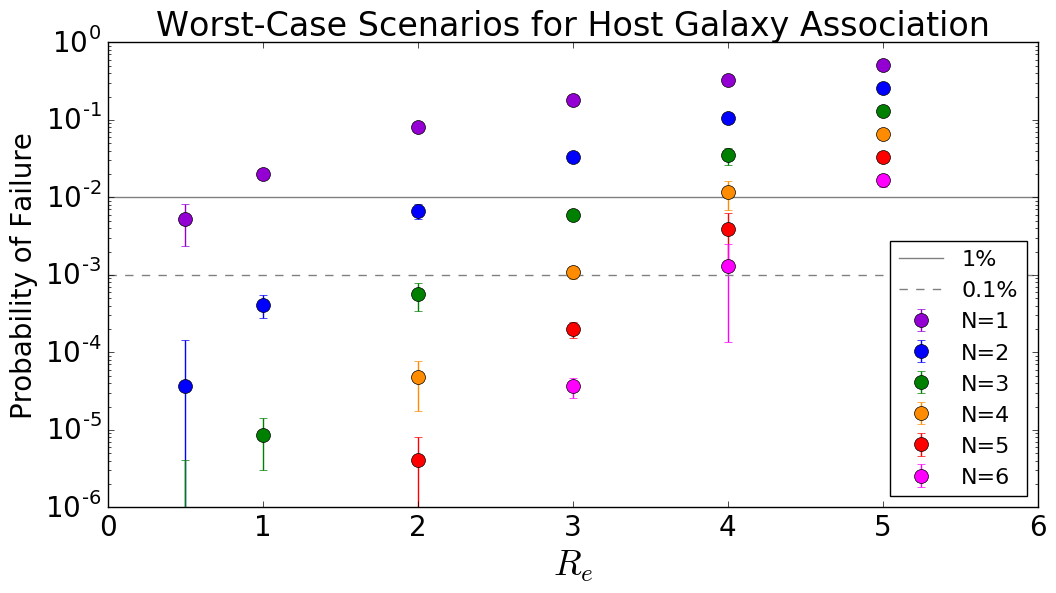
\includegraphics[width=12cm]{hg_P_vs_Re.png}
\caption{The probability that a transient will fail to be associated with a large ($R_e=10$ kpc) nearby host galaxy due to background interlopers, as a function of the transient's offset in effective radii from galaxies in the vicinity (including the true host), where ``failure" means the true host's separation distance is not in the top $N$ nearest galaxies. \textbf{This is a ``worst case scenario" because it applies to an very large nearby galaxy, and all background galaxy radii estimates are upper limits} (as described in the text). Error bars show the standard deviation from the 100 randomly-generated sets of background galaxies. \label{fig:pfail}}
\end{center}
\end{figure}
